\chapter{Valore Atteso: Integrale Rispetto ad una Misura di Probabilità}

Nel capitolo precedente abbiamo studiato profondamente l'integrazione di Lebesgue rispetto ad una misura $ \mu $ che sia $\sigma$--finita. In questo capitolo riformuleremo tutte le nozioni viste precedentemente, ma nel caso in cui si integri rispetto ad una misura di probabilità.

\medskip
\noindent È così che andremo a definire il \textit{valore atteso }, che rappresenta, in sostanza, la media dei possibili valori di una variabile aleatoria reale, pesata secondo le rispettive probabilità di occorrenza.\\
\\
In questo capitolo costruiremo progressivamente la nozione di valore atteso. Il 
modus operandi sarà lo stesso che è stato utilizzato nel capitolo precedente: definiremo prima l'integrale (o valore atteso) per variabili aleatorie semplici, poi per variabili non negative, per poi arrivare ad una generalizzazione a variabili generiche.

\begin{esempio}
    Qualora una variabile aleatoria $X$ rappresenti la distribuzione di massa di un oggetto, il valore atteso $E[X]$ ne individua il baricentro.
\end{esempio}
\section{Valore atteso per Variabili Aleatorie Semplici}
\begin{definizione}
    Sia $X:(\Omega, \mathcal{A}, \mathbb{P})\to (\mathbb{R}, \mathcal{B})$ una variabile aleatoria semplice, ossia che assume un numero finito di valori $x_1, ..., x_n\geq0$. Questa può essere scritta come:
    \[X(w) = \sum_{k=1}^n x_k\;\mathbb{I}_{A_k}(w) =  \sum_{k=1}^n x_k\;\mathbb{I}_{(X = x_k)}(w)\]
    Allora possiamo definire il valore atteso di $X$ come:
    \[E[X] = x_1\cdot \mathbb{P}(A_1)+ \cdots +x_n\cdot \mathbb{P}(A_n) = \sum_{k=1}^n x_k\cdot\mathbb{P}(A_k)\quad \Rightarrow\quad E[X] :=\int_\Omega X(w)\;\mathbb{P}(dw) =  \int_\Omega X\;d\mathbb{P}\]
\end{definizione}

\section{Generalizzazione a Variabili Aleatorie Generiche}
\noindent Come afferma la Proposizione \ref{prop:6.4}, data una funzione positiva semplice (o elementare), allora possiamo trovare una successione di funzioni elementari che converge alla funzione in maniera crescente. Utilizziamo la Definizione \ref{def:6.5} per estendere il concetto di valore atteso a variabili aleatorie positive, utilizzando la successione che avevamo già introdotto.

\begin{definizione}[\text{$E[X]$ per Variabili Positive}]
    Sia $X:\Omega\to[0, +\infty]$ una variabile aleatoria positiva, allora definiamo il valore atteso come:
    \[E[X] \overset{\ref{def:6.5}}{=} \lim_{n\to+\infty} E[X_n]  = \lim_{n\to+\infty} \sum_{k=1}^{n2^n - 1} \frac{k}{2^n} \cdot \mathbb{P}\left(\frac{k}{2^n}\leq X<\frac{k+1}{2^n}\right) + n\cdot \mathbb{P}(X\geq n)\]
    Dove $X_n = \begin{cases}
        \frac{k}{2^n}, \quad &\frac{k}{2^n}\leq X<\frac{k+1}{2^n}\\
        n, &X\geq n
    \end{cases}; \quad k = 0, ..., n2^n-1$
\end{definizione}

\noindent Si osservi già che se $\mathbb{P}(X=+\infty) = c>0\quad \Rightarrow\quad E[X] = +\infty, \;$ infatti:
\[(X>+\infty)\subseteq(X\geq n) \quad \Rightarrow\quad c = \mathbb{P}(X=+\infty) \leq \mathbb{P}(X\geq n)\]
e allora:
\begin{align*}
    E[X_n] &= \sum_{k=1}^{n2^n - 1} \frac{k}{2^n} \cdot \mathbb{P}\left(\frac{k}{2^n}\leq X<\frac{k+1}{2^n}\right) + n\cdot \mathbb{P}(X\geq n) \\
    & \geq n\cdot \mathbb{P}(X\geq n) \geq n\cdot \mathbb{P}(X = +\infty) = n\cdot c \\
    \\
    \Rightarrow\qquad E[X] &= \lim_{n\to+\infty} E[X_n] \geq \lim_{n\to+\infty} nc = +\infty
\end{align*}

\bigskip
\noindent Di nuovo, come abbiamo fatto nel capitolo precedente, scomponiamo una V.A. reale nella sua parte positiva e negativa, riuscendo così a definire il suo integrale, finito od infinito.

\begin{definizione}[Ammissione del Valore Atteso]
    Sia $X:\Omega\to\mathbb{R}$ una variabile aleatoria, e siano $X_+:=X\vee0, \;X_-:=(-X)\vee 0$. Allora $X$ ammette Valore Atteso se:
    \[E[X_+]<+\infty \qquad \text{oppure}\qquad E[X_-]<+\infty\]
    In tal caso:
    \[E[X] = E[X_+] - E[X-] = \begin{cases}
        +\infty\\
        |\text{c}| < +\infty\\
        -\infty
    \end{cases}\]
\end{definizione}

\begin{definizione}[Integrabilità di $X$]
    Sia $X:\Omega\to\mathbb{R}$ una variabile aleatoria. Questa si definisce integrabile se:
    \[E[X_+]<+\infty \qquad \text{e}\qquad E[X_-]<+\infty\]
    In tal caso:
    \[E[X] = E[X_+] - E[X-] \in \mathbb{R}\]
\end{definizione}

\bigskip
\noindent Possiamo di nuovo ridefinire lo spazio $\mathcal{L}^1$ su uno spazio di probabilità:
\begin{align*}\mathcal{L}^1(\Omega, \mathcal{A}, \mathbb{P}) & = \set{X:\Omega \to \mathbb{R}\;\;  V.A.\;\big|\; E\left[|X|\right]<+\infty}\\
& =\set{X:\Omega \to \mathbb{R}\;\;  V.A.\;\big|\; \int_\Omega|X|\;d\mathbb{P}<+\infty}
\end{align*}

\newpage
\section{Proprietà del Valore Atteso}
Cerchiamo di riassumere tutte le proprietà che possiede $E[X]$, ed andiamo a definirne di ulteriori rispetto all'integrazione rispetto ad una misura $\sigma$--finita.
\begin{teorema}[Proprietà del Valore Atteso]
    Riassumiamo tutte le proprietà del Valore Atteso $E[X]$:
    \begin{enumerate}
        \item $\mathcal{L}^1(\Omega, \mathcal{A}, \mathbb{P})\;$ è uno spazio vettoriale: \[\quad \forall X, Y\in\mathcal{L}^1(\Omega, \mathcal{A}, \mathbb{P}), \; \alpha, \beta \in \mathbb{R} \quad \Rightarrow\quad \alpha X + \beta Y \in \mathcal{L}^1(\Omega, \mathcal{A}, \mathbb{P})\]
        Inoltre, $E :\mathcal{L}^1(\Omega, \mathcal{A}, \mathbb{P})\longrightarrow\mathbb{R}\;$ è una mappa lineare, positiva e monotona:
        \begin{itemize}
            \item $E[\alpha X + \beta Y] = \alpha E[X] + \beta E[Y]$ \hfill \textit{(Lineare)}
            \item $\forall X\geq0 \quad \Rightarrow \quad E[X]\geq 0$ \hfill \textit{(Positiva)}
            \item $Y\in \mathcal{L}^1, \;Y\geq X\geq 0 \Rightarrow X\in \mathcal{L}^1\quad E[Y] \geq E[X]\geq 0 \quad$ \hfill \textit{(Monotona)}
        \end{itemize}

    \item $X\geq 0, \;E[X] = 0 \quad \Rightarrow\quad X =0\; $ quasi certamente
    \item $X, Y \geq0, \; \alpha, \beta \geq0 \quad \Rightarrow\quad \alpha E[X] + \beta E[Y]$
    \item $X\in \mathcal{L}^1(\Omega, \mathcal{A}, \mathbb{P})\; \quad \iff \quad |X| \in \mathcal{L}^1(\Omega, \mathcal{A}, \mathbb{P})\;\text{ e }\; \left|E[X]\right| \leq E[|X|]$
    \item $X = Y\;$ q.c. $\quad \Rightarrow\quad E[X] = E[Y]$
    \item Convergenza Monotona (Beppo Levi):\\
    Sia \(\;(X_n)_{n\geq1}\;\text{ tale che }\; X_{n+1} \geq X_n\geq 0\;\text{quasi certamente},\;X\geq0\;\text{ V.A., tali che:}\;\underset{n\to\infty}{\lim} X_n = X\; \text{ quasi certamente}:\)
    \[\Rightarrow\quad \lim_{n\to\infty}E[X_n] = E[X] = E\left[\lim_{n\to\infty}X_n \right]\]
    \item Convergenza Dominata (Lebesgue):
    Sia $(X_n)_{n\geq1},\; X \;\text{ V.A., tali che:}\; \underset{n\to\infty}{\lim} X_n = X\; \text{ quasi certamente}\;$ e si abbia che $\;\exists Y\in \mathcal{L}^1:\; |X_n|\leq Y\;$ quasi certamente:
    \[\Rightarrow\quad X_n, X\in \mathcal{L}^1\qquad \text{e}\qquad \lim_{n\to\infty}E[X_n] = E[X] = E\left[\lim_{n\to\infty}X_n \right]\]
    Ossia che:$\quad E\left[\underset{n\to\infty}{\lim}|X_n-X| \right] = 0$
    \end{enumerate}
\end{teorema}

Tutti i risultati di questo teorema valgono per una $\mu$ generica $\sigma$--finita, e quindi anche nel caso particolare in cui $\Omega = \mathbb{R}, \mathcal{A}=\mathcal{B}, \mu=\mathbb{P}$. Inoltre tutti i risultati che valgono per i valori attesi $E[X]$, valgono quasi certamente, questo significa che se $Y = X$ q.c. valgono anche per $E[Y]$.\\
\\
Siccome in questo capitolo stiamo trattando il caso specifico in cui $\mu = \mathbb{P}$, e la probabilità è una misura finita e non semplicemente  $\sigma$--finita, l'integrale (quindi $E[X]$) gode di altre proprietà specifiche:

\begin{corollario}
\label{cor:7.6}
    Siccome $\mathbb{P}$ è una misura finita, allora $E[X]$ gode anche delle seguenti proprietà:
    \begin{enumerate}
        \item [8.] $X = c\;$ quasi certamente $\quad \Rightarrow\quad X\in\mathcal{L}^1\;$ e $\;E[X] = c$
        \item [9.] $E[X]>0 \quad \Rightarrow\quad \mathbb{P}(X>0) >0$
        \item [10.] $E[|X|] = E[X_+] + E[X_-]$
        \item [11.]$ a\leq X\leq b\;$ quasi certamente $\quad \Rightarrow\quad a\leq E[X]\leq b$
    \end{enumerate}
    
    \begin{dimostrazione}
        \begin{enumerate}
        \item [8.] $X = c\;$ quasi certamente $\quad \overset{7.5\;(5)}{\Rightarrow}\quad E[X] = E[c] = c\cdot\mathbb{P}(\Omega) = c$
        \item [9.] $E[X] = E[X_+] - E[X_-]>0\quad \Rightarrow\quad E[X_+]>E[X_-]\geq0.\;$ Allora $E[X_+]>0$\\$\Rightarrow\quad\int_{\{X>0\}}X\;d\mathbb{P}>0\quad \Rightarrow\quad \mathbb{P}(X>0)>0$
        \item [10.] Ovvia.
        \item [11.] Sia  $a\leq X\leq b\quad \Rightarrow\quad |X|\leq |a| \vee |b| \quad \overset{7.5\;(1)+(8)}{\Rightarrow} E[|X|] \leq E\left[|a| \vee |b|\right] = |a| \vee |b|$.\\
        Di conseguenza $X\in\mathcal{L}^1,\;$ quindi è lecito calcolarne il valore atteso. \\
        Dato che $E[X-a]\geq 0 \quad \Rightarrow\quad E[X]\geq a$. Stesso raginamento per $b$
    \end{enumerate}
    \end{dimostrazione}
\end{corollario}

\noindent Due considerazioni importanti su questo teorema e corollario:
\begin{itemize}
    \item Tutte le uguaglianze o disequazioni che riguardano $E[\cdot]$, non sono intese in senso ``quasi certo'', bensì in senso certo. Questo perché $E[\cdot]\in\mathbb{R}$, non è una funzione.
    \item Si noti come le proprietà esposte nel Corollario \ref{cor:7.6} siano intuitivamente valide solo perchè $\mathbb{P}(\Omega) = 1$. Per esempio le costanti (8.) non si integrano su illimitati di $\mathbb{R}$ rispetto a $m$, e nemmeno le funzioni limitate (11.) sono sempre integrabili su domini illimitati.
\end{itemize}

\bigskip
\noindent
\begin{tikzpicture}
  \draw[dashed] (0,0) -- (\textwidth,0);
\end{tikzpicture}\\
\\
Prendiamo in esame un'applicazione estremamente utile, ovvero dove $\Omega$ è discreto. \textit{Esiste una maniera operativa per poter calcolare il valore atteso, ``senza passare'' dall'integrale?}\\
\\
Sia $\Omega$ discreto, ossia: $\Omega = \{w_n:n\geq1\}$. Si prenda $\;\mathcal{A} = 2^\Omega$ e $X\in\mathcal{L}^1$. Allora per il Teorema \ref{th:2.7} si ha che $\;\mathbb{P}\leftrightarrow (p_n)_{n\geq1}:\quad p_n = \mathbb{P}(\{p_n\}).$ \\
Allora è vero che:
\[\boxed{E[X] = \int_\Omega X\;d\mathbb{P} = \sum_{n\geq1} X(w_n)\cdot p_n}\]

\begin{dimostrazione}
    Sia $X:\Omega\to[0, +\infty]$ ed $\Omega$ numerabile. Definiamo la seguente successione di funzioni:
    \[X_k(w) = \begin{cases}
        X(w), \quad & \text{se } w\in \{w_1, ..., w_k\}\\
        0 & \text{se } w\notin\{w_1, ..., w_k\}
    \end{cases}\]
\begin{figure}[H]
\centering
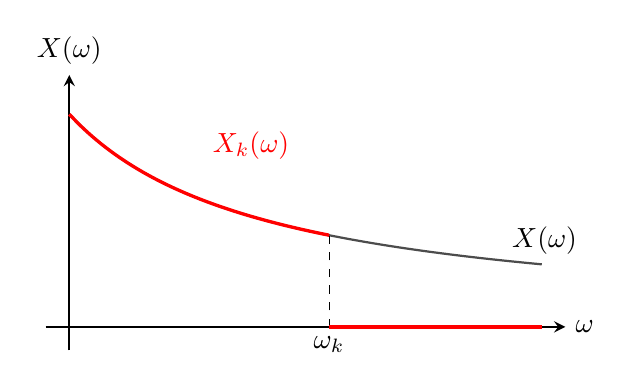
\begin{tikzpicture}[>=stealth, scale=1]

  % --- Assi ---
  \draw[->, thick] (-0.3,0) -- (6.3,0) node[right] {$\omega$};
  \draw[->, thick] (0,-0.3) -- (0,3.2) node[above] {$X(\omega)$};

  % --- Curva continua X(w) ---
  \draw[domain=0:6, smooth, variable=\x, thick, black!70]
    plot ({\x}, {2.7/(1+0.4*\x)});
  \node[right] at (5.5,1.1) {$X(\omega)$};

  % --- Parte di X_n coincidente con X ---
  \draw[very thick, red, domain=0:3.3, smooth, variable=\x]
    plot ({\x}, {2.7/(1+0.4*\x)});
  \node[red, above right] at (1.7,2.0) {$X_k(\omega)$};

  % --- Linea tratteggiata verticale in ω_n ---
  \draw[dashed] (3.3,0) -- (3.3,{2.7/(1+0.4*3.3)});
  \node[below] at (3.3,0) {$\omega_k$};

  % --- Parte nulla di X_n ---
  \draw[very thick, red] (3.3,0) -- (6,0);

\end{tikzpicture}
\end{figure}
$X_k$ può quindi assumere un numero finito di valori, quindi:
\[E[X_k] = \sum_{h=1}^k X(w_h)p_h\]
Dove:
\begin{itemize}
    \item $X_k$ è una successione di funzioni crescenti, in quanto $X_{k+1} \geq X_k$, \item Per costruzione: $\underset{k\to+\infty}{\lim}X_k(w) = X(w)\quad \forall w\in \Omega$
\end{itemize}
Si può quindi usare il Teorema di Beppo Levi:
\[
    E[X] = \lim_{k\to+\infty}E[X_k] = \lim_{k\to+\infty}\sum_{h=1}^k X(w_h)\mathbb{P}(w_h) = \lim_{k\to+\infty}\sum_{h=1}^k X(w_h)p_h
\]
In particolare si ha che: 
\[E[|X|] = \sum_{h=1}^\infty \left|X(w_h)\right|p_h\]
Di conseguenza: $\;X\in \mathcal{L}^1(\Omega, 2^\Omega, \mathbb{P})\quad \iff\quad \sum_{h=1}^\infty \left|X(w_h)\right|p_h<+\infty$
\end{dimostrazione}

\bigskip
\noindent Questa applicazione al caso discreto è molto utile in campo applicativo, in quanto se, per esempio, si ha una variabile aleatoria distribuita come una Poisson, allora possiamo calcolare in maniera estremamente facile il suo valore atteso:\\
\\
Sia $\Omega = \mathbb{N};\; \mathcal{A} = 2^\mathbb{N}; \; \mathbb{P} = \text{ Poisson}(\lambda), \; \lambda>1,\;$ ovvero che $\;p_k = \frac{e^{-\lambda}\lambda^k}{k!}\;\forall k\geq0$.\\
Si consideri la variabile aleatoria $X:\Omega\to\mathbb{R}:\; X(k) = k!, \;k\in\mathbb{N}$. Allora possiamo calcolare $E[X]$ come segue:
\[E[X] = \sum_{k=0}^\infty X(k)\cdot p_k = \sum_{k=0}^\infty k!\;p_k = e^{-\lambda} \sum_{k=0}^\infty\lambda^k = +\infty\]
Abbiamo quindi calcolato in questo caso che il valore atteso è $\infty$, anche se $\mathbb{P}(X = +\infty) = 0$.

\medskip
\noindent Abbiamo appena dimostrato che anche se $X$ assume valori reali, non è detto che il valore atteso sia finito, ma soprattutto che:
\[\mathbb{P}(X = +\infty) = 0 \quad \not\Rightarrow \quad E[X]  < + \infty\]


\bigskip
\noindent
\begin{tikzpicture}
  \draw[dashed] (0,0) -- (\textwidth,0);
\end{tikzpicture}\\
\\
Ovviamente anche la Definizione \ref{def:6.12} è valida nel caso in cui si integri rispetto ad una misura di probabilità:
\begin{definizione}
\label{def:7.7}
    $\forall A\in\mathcal{A}: $ 
    \[\int_AX(w) \;d\mathbb{P} = \int_\Omega (X\mathbb{I})_A\;d\mathbb{P} = E[X\mathcal{I_A}]\]
    In particolare:\[\forall A\in\mathcal{A}:\qquad \mathbb{P}(A) = 1\cdot \mathbb{P} (A)+ 0\cdot \mathbb{P}(A^c) = \int_\Omega \mathbb{I}_A\;d\mathbb{P} = \int_A d\mathbb{P} = E[\mathbb{I}_A]\]
\end{definizione}

\begin{teorema}[Disuguaglianza di Markov]
\label{th:dismark}
    Sia $(\Omega, \mathcal{A}, \mathbb{P})$ uno spazio di probabilità, e sia $\;X:\Omega\to\mathbb{R}$ una variabile aleatoria reale.
    \[\Rightarrow\quad \forall a>0:\qquad \boxed{\mathbb{P}\left(|X|\geq a\right)\leq \frac{E[\,|X|\,]}{a}}\]
    \begin{dimostrazione}
        Grazie alla Definizione \ref{def:7.7} sappiamo che:
        \[\mathbb{P}(|X|\geq a) = E\left[\mathbb{I}_{(|X|\geq a)}\right]\]
        Inoltre, affinché $w \in (\left|X|\geq a\right) \quad \Rightarrow \quad |X(w)|\geq a \iff \frac{|X(w)|}{a}\geq 1$. \\
        Quindi l'identità dell'insieme $|X|\geq a$ risulta essere:
        \[\mathbb{I}_{(|X|\geq a)}(w) = \begin{cases}
            1\leq \frac{|X(w)|}{a}, \quad &\text{se } w\in(|X|\geq a)\\
            0, &\text{se } w\notin(|X|\geq a)
        \end{cases}\]
        Dunque:
        \[\mathbb{I}_{(|X|\geq a)}(w) \leq \frac{|X(w)|}{a}\cdot\mathbb{I}_{(|X|\geq a)}\overset{\mathbb{I}_{(|X|\geq a)}\leq 1}{\leq} \frac{|X(w)|}{a}\cdot 1\]
        Di conseguenza, per monotonia del valore atteso avremo che:
        \[\mathbb{P}(|X|\geq a) = E[\mathbb{I}_{(|X|\geq a)}]\leq E\left[\frac{|X|}{a}\right] = \frac{E[|X|]}{a}\]
    \end{dimostrazione}
\end{teorema}

\section{Spazio $L^p$}

Consideriamo due variabili aleatorie $X, Y : \Omega \to \mathbb{R}$ definite sullo stesso spazio di probabilità $(\Omega, \mathcal{A}, \mathbb{P})$.  
Può accadere che
\[
X(w) \neq Y(w) \quad \text{per alcuni } w \in \Omega,
\]
ma che le due siano uguali quasi certamente, cioè \(\;\mathbb{P}(X = Y) = 1.\)
In termini di misura, come abbiamo già detto, questo significa che la differenza tra $X$ e $Y$ è rilevante solo su un insieme di probabilità nulla.

\medskip
\noindent
Tuttavia, molte proprietà fondamentali, come
\[
E(X) = \int_\Omega X\,d\mathbb{P},
\]
non cambiano se si modifica $X$ su un insieme di probabilità zero.  
Se lavorassimo direttamente con le funzioni, potremmo quindi avere due funzioni \emph{diverse come oggetti puntuali}, ma che rappresentano la stessa ``realtà probabilistica'', poiché hanno la stessa integrale, la stessa distribuzione e coincidono quasi ovunque.

\medskip

\noindent
Per questo motivo, nella teoria della misura e della probabilità non ha senso distinguere funzioni che differiscono solo su insiemi di misura nulla.  
Si nota a questo punto che $X\overset{\text{q.c.}}{=}Y$ è una vera e propria \textbf{relazione di equivalenza}, in quanto è riflessiva, simmetrica e transitiva.\\
\\
Ha senso andare a lavorare non più con le funzioni, ma con le classi di equivalenza. Possiamo quindi definire un nuovo spazio sul quale lavorare:
\begin{definizione}
    Si definisce la classe di equivalenza rispetto alla relazione di equivalenza quasi certa:
    \[
        [X] = \{\, Y \in \mathcal{L}^1 : Y = X \text{ q.c.} \,\}.
    \]
    L'insieme $\mathcal{L}^1$ quozientato rispetto all'uguaglianza quasi certa, si definisce spazio \[L^1 = \mathcal{L}^1 /\sim\; = \set{\text{Insieme delle classi di equivalenza }[X] \mid X\in \mathcal{L}^1}\]
\end{definizione}

$L^1$ è quindi l'insieme di tutte le classi di equivalenza di funzioni integrabili (in senso di Lebesgue) che coincidono quasi certamente.  
In altre parole, in $L^1$ non lavoriamo più con le singole funzioni, ma con le classi di equivalenza, poiché le differenze su insiemi di misura nulla non hanno effetto né sull'integrale, né sulle proprietà analitiche rilevanti.
\[
\boxed{\text{In teoria della misura e della probabilità, } L^1 \text{ è lo spazio naturale dove vive l'integrale di Lebesgue.}}
\]

\faWarning $\;$ Abbiamo quindi capito che $\mathcal{L}^1$ e $L^1$ sono due insiemi ben differenti, tuttavia in questo corso andremo ad utilizzare un piccolo \textit{abuso di notazione}: scriveremo infatti che $X\in L^1$, al posto che scrivere $[X]\in L^1$.

\medskip
\noindent È come se utilizzassimo la scrittura
\[L^1(\Omega, \mathcal{A}, \mathbb{P}) = \set{X:\Omega\to\mathbb{R} \text{ V.A. } \mid E[|X|]<+\infty}\]
ma tenendo sempre ben saldo a mente che non stiamo lavorando con funzioni, ma con le loro classi di equivalenza \faWarning\\
\\
Osserviamo inoltre che $L^1$ è  uno spazio vettoriale, ossia che:
\[X_1 \overset{\text{q.c}}{=} X_2;\;Y_1 \overset{\text{q.c}}{=} Y_2; \; X_1, X_2, Y_1, Y_2 \in L^1 \quad \Rightarrow\quad \forall \alpha, \beta \in \mathbb{R}\quad \alpha X_1 + \beta Y_1 = \alpha X_2 + \beta Y_2\]

\noindent Possiamo estendere questo concetto ad uno più generale:
\begin{definizione}
    Definiamo lo spazio $\mathcal{L}^p, \;\forall 1\leq p < +\infty$ come segue:
    \[\mathcal{L}^p = \set{X:\Omega\to\mathbb{R} \text{ V.A. }\mid E[|X|^p]<+\infty}\]
    Allo stesso modo di prima definiamo:
    \[L^p = \set{\text{Insieme delle classi di equivalenza }[X] \;\big|\; |X|^p\in \mathcal{L}^1}\]
    \faWarning $\;$ Con lo stesso abuso di notazione precedente, utilizzeremo
    \[L^p(\Omega, \mathcal{A}, \mathbb{P}) = \set{X:\Omega\to\mathbb{R} \text{ V.A. } \mid E\big[|X|^p\big]<+\infty}\]
\end{definizione}
Come è facile immaginarsi, se una variabile aleatoria è costante $X = c$, allora $X\in L^p, \;\forall1\leq p<+\infty$ e $E[|X|^p] = |c|^p$

\begin{teorema}
    Valgono le seguenti proprietà, nel caso in cui integriamo per una misura di probabilità:
    \begin{enumerate}
        \item $L^2 =  \set{X:\Omega\to\mathbb{R} \text{ V.A. }\mid E[|X|^2]<+\infty}\subseteq L^1$
        \item $L^2$ è  uno spazio vettoriale: $\quad X, Y\in L^2\quad \Rightarrow\quad \forall\alpha, \beta\in\mathbb{R}\quad \alpha X+\beta Y\in L^2$
        \item Disuguaglianza di Cauchy--Schwarz:\[X, Y\in L^2\quad \Rightarrow\quad X\cdot Y\in L^1\;\text{ e }\; \boxed{\big|E[X\cdot Y]\big|\leq \sqrt{E[X^2]\cdot E[Y^2]}}\]
        \item $\forall 1\leq p\leq q<+\infty$ vale che $L^q\subseteq L^p$
    \end{enumerate}
\end{teorema}

Si presti particolare attenzione che questo teorema è valido solo nel caso in cui si sta integrando rispetto ad una misura di probabilità (la quale è una misura finita). Si possono  definire gli spazi $L^p$ su un generico spazio di misura $(E, \mathcal{E}, \mu)$. Non è infatti detto che se si prende una misura $\sigma$--finita allora, per esempio, $L^p\subseteq L^q\;$ se $\;p\leq q$.

\begin{esempio}
    Si prenda in esame la funzione $f(x) = \frac{1}{x}$ nel dominio $(1, +\infty) =:D$, e la si integri rispetto la misura di Lebesgue $m$.\\
    Avremo che:
    \[\int_{(1, +\infty)} \left| f(x)\right|\;dm = \int_1^{+\infty}  \frac{1}{x}\;dx = +\infty \qquad \Rightarrow\qquad f\notin L^1(D, \mathcal{B}(D
    ), m)\]
    Tuttavia:
    \[\int_{(1, +\infty)} \left| f(x)\right|^2\;dm = \int_1^{+\infty}  \frac{1}{x^2}\;dx < +\infty \qquad \Rightarrow\qquad f\in L^2\left(D, \mathcal{B}(D
    ), m\right)\]
    Abbiamo dimostrato che non è vero che $L^2\subseteq L^1$ nel caso in cui si integri rispetto ad una misura $\sigma$--finita.
\end{esempio}

\section{Varianza}
La varianza è una delle grandezze fondamentali della teoria della probabilità e della statistica, poiché misura la \textbf{dispersione} dei valori assunti da una variabile aleatoria rispetto al suo valore medio. Se il valore atteso descrive il ``centro'' della distribuzione, la varianza ne quantifica invece la \textbf{variabilità}, 
indicando quanto i possibili esiti si discostano, in media, da tale centro.

\medskip

Comprendere la varianza significa quindi analizzare quanto è stabile o incerta una grandezza aleatoria: una varianza piccola implica che i valori osservati sono concentrati attorno alla media, mentre una varianza elevata segnala una forte variabilità e dunque una maggiore incertezza.

\begin{figure}[H]
\centering
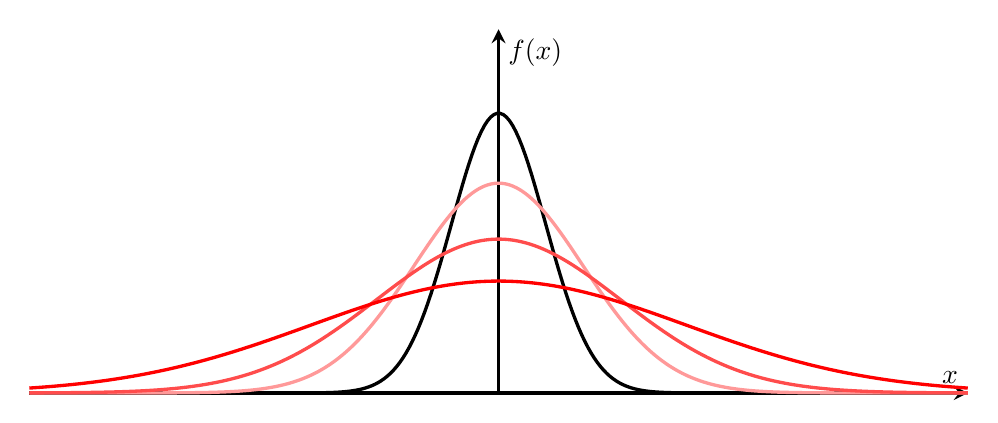
\begin{tikzpicture}
\begin{axis}[
    width=13.5cm, height=6.2cm,
    domain=-5:5, samples=300,
    axis lines=middle,
    axis line style={very thick},
    xlabel={$x$}, ylabel={$f(x)$},
    xtick=\empty, ytick=\empty,
    clip=false,
    enlargelimits=false,
    xmin=-5, xmax=5, ymin=0, ymax=1.3,
]
% --- Gauss con stessa media (0) e varianza crescente (sigma^2) ---
% (non serve normalizzare: ci interessa solo la forma)
\addplot[black, very thick]      {exp(-x^2/(2*0.5^2))};  % varianza piccola
\addplot[black, very thick, red!40]      {0.75*exp(-x^2/(2*0.9^2))};
\addplot[black, very thick, red!70]      {0.55*exp(-x^2/(2*1.3^2))};
\addplot[black, very thick, red]      {0.40*exp(-x^2/(2*2.0^2))}; % varianza grande

\end{axis}
\end{tikzpicture}
\caption{Stessa media, varianza crescente: la curva si allarga al crescere della dispersione.}
\end{figure}

Diamo quindi la definizione formale di Varianza.

\begin{definizione}[\faWarning]
    Sia $(\Omega, \mathcal{A}, \mathbb{P})$ uno spazio di probabilità, e sia $X\in L^2(\Omega, \mathcal{A}, \mathbb{P})$. Definiamo la Varianza di $X$ il numero:
    \[Var(X) := \sigma^2 :=E\left[(X-E[X])^2\right]\]
\end{definizione}
Si osservi che dato che stiamo integrando rispetto ad una misura di probabilità, allora dato che $X\in L^2$ implica che $X\in L^1$, e quindi $E[X]<+\infty$.

\begin{teorema}[Proprietà della Varianza]
    Per ogni variabile aleatoria $X\in L^2$, valgono le seguenti proprietà:
    \begin{enumerate}
        \item $Var(X) = E\left[(X-E[X])^2\right] \geq 0$
        \item $Var(X) = 0\quad \iff \quad \exists \,c\in \mathbb{R}\;\text{ tale che }\; X \overset{\text{q.c.}}{=} c \; \text{ e } \;E[X] = c \quad \iff\quad P^X\sim \delta_c$
        \item Disuguaglianza di Chebychev:\\
        \[\boxed{\mathbb{P}(|X-E[X]|\geq a)\leq \frac{\sigma^2}{a^2}}\quad \forall a>0\]
        \item $Var(X) = E[X^2] - E[X]^2$
        \item $Var(aX+b) = a^2Var(X)\quad \forall a, b\in\mathbb{R}$
    \end{enumerate}
    \begin{dimostrazione}
    Dimostriamo solo la 3. e 5.
    \begin{enumerate} 
        \item [3.] Vedendo che $(|X-E[X]|\geq a) = (|X-E[X]|^2\geq a^2)$, possiamo usare la disuguaglianza di Markov (Teorema \ref{th:dismark}) con $Y = |X-E[X]|^2 = (X-E[X])^2$:
        \begin{align*}\mathbb{P}(|Y|\geq a^2)\leq \frac{E[Y]}{a^2}\quad \iff\quad\mathbb{P}\left((X-E[X])\geq a\right) & = \mathbb{P}\left((X-E[X])^2\geq a^2\right)\\
        &\leq \frac{E\left[(X-E[X])^2\right]}{a^2} = \frac{\sigma^2}{a^2}\end{align*}
        \item [5.] $Var(aX+b) = E\left[(aX+b - E[aX+b])^2\right] = E\left[\left(aX-aE[X]\right)^2\right] = a^2Var(X)$ 
    \end{enumerate}
    \end{dimostrazione}
\end{teorema}

\section{Regola del Valore Atteso}

Vediamo adesso un metodo per calcolare in modo concreto il valore atteso nelle applicazioni reali: la regola del valore atteso

\medskip
\noindent Questa regola ci permette di semplificare il calcolo del valore atteso quando la variabile aleatoria può essere espressa in funzione di un’altra. Si tratta di uno strumento fondamentale nella pratica, poiché consente di passare da un approccio puramente teorico a uno operativo, applicabile a problemi reali di previsione, stima e decisione.\\
\\
Se guardiamo al problema con solo la "lente della teoria della misura", allora quello
che stiamo per fare è definire un modo per calcolare l'integrale di funzioni misurabili e delle loro composizioni: nulla di più, nulla di meno.

\begin{definizione}[\faWarning $\;$ Regola del valore Atteso]
\label{def:regE}
    Sia $(\Omega, \mathcal{A}, \mathbb{P})$ uno spazio di probabilità, e $(E, \mathcal{E})$ uno spazio misurabile. Si considerino $\;X:\Omega\to\mathbb{R}$ variabile aleatoria e $\;h:E\to\mathbb{R}$ oppure $[0, +\infty]$ misurabile.\\
    Allora vale che:
    \begin{enumerate}
        \item $h(X) \in L^1 (\Omega, \mathcal{A}, \mathbb{P})\quad \iff \quad h \in L^1(E, \mathcal{E}, P^X)$
        \item Sia nel caso in cui $h:E\to[0, +\infty]$, sia nel caso in cui $h\in L^1(\cdot)$, si ha che:
        \[E\left[h(X)\right]= \boxed{\int_\Omega h(X) \;d\mathbb{P} = \int_E h\;dP^X} := E^X(h)\] 
    \end{enumerate}
\end{definizione}

Questo teorema è molto importante nel calcolo del valore atteso, poiché afferma
che svolgere l’integrale su $\Omega$ equivale a calcolarlo su $E$. Infatti, in molti casi il dominio $\Omega$ può essere un insieme astratto composto da oggetti qualsiasi,
su cui non è definita l’integrabilità.

\medskip
\noindent Imponendo $E = \mathbb{R}$, il calcolo si trasforma in un integrale su $\mathbb{R}$,rendendolo possibile o comunque più agevole.
\begin{esempio}
    Prendiamo per esempio il caso in cui $X:(\Omega, \mathcal{A}, \mathbb{P})\to(\mathbb{R}, \mathcal{B})\;$ e $\;h:\mathbb{R}\to\mathbb{R}$.

\begin{figure}[H]
\centering
\begin{tikzpicture}[x=1.5cm,y=1.5cm,>=stealth, font=\small]

% --- Spazio di partenza: (Omega, A, P)
\draw[very thick] (-3,0) rectangle (-1,2);
\node[below=2pt of {(-2,0)}, yshift=0.1cm] {$(\Omega,\mathcal{A},\mathbb{P})$};

% --- Freccia X : Omega -> R
\draw[->, thick] (-0.9,1.1) .. controls (0,1.7) and (2,1.7) .. (2.9,1.1);
\node at (1,1.9) {$X$};

% --- Asse dei reali: (R, B, P^X)
\draw[->, very thick] (3,0) -- (3, 2);
\node at (3,2.3) {$\mathbb{R}$};
\node[below=2pt of {(3,0)}, yshift=0.1cm] {$(\mathbb{R},\mathcal{B},P^X)$};

% --- E(X)
\fill (3,1) circle (1.4pt);
\node[left] at (2.7,1) {$E[X]$};
\node at (1.5,0.5) {$\displaystyle E[X] = \int_\Omega X(w)\, d\mathbb{P}(w)$};

% --- Freccia h: R -> R
\draw[->, thick] (3.3,1.1) .. controls (4,1.7) and (6,1.7) .. (6.9,1.1);
\node at (5,1.9) {$h(X)$};

% --- Secondo asse dei reali
\draw[->, very thick] (7,0) -- (7, 2);
\node at (7,2.3) {$\mathbb{R}$};
\node[below=2pt of {(7,0)}, yshift=0.1cm] {$(\mathbb{R},\mathcal{B})$};

% --- E^X(h)
\fill (7,1) circle (1.4pt);
\node[left] at (6.6,1) {$E[h(X)]$};

% --- Formule a destra
\node[right] at (4.5,0.5) {$\displaystyle E^X(h) = \int_{\mathbb{R}} h\, dP^X$};
\end{tikzpicture}
\end{figure}
\end{esempio}

\bigskip
\noindent Se si assume che $h=\text{Id}(x):\mathbb{R}\to\mathbb{R}$ definita come $\text{Id}(x) = x$, allora abbiamo un modo estremamente concreto di calcolare il valore atteso di una variabile aleatoria, ossia:
\[E[h(X)] = \int_\Omega \text{Id}(X)\;d\mathbb{P} = \int_\mathbb{R} \text{Id}(x) \;dP^X = \int_\mathbb{R} x \;dP^X\quad \Rightarrow \quad \boxed{E[X] = \int_\mathbb{R}x\;dP^X}\]

\bigskip
\noindent Questo teorema ci permette di capire un altro fatto fondamentale: \textbf{il valore atteso è una proprietà esclusivamente delle legge} di una variabile aleatoria. Presi infatti $X_1:(\Omega_1, \mathcal{A}_1, \mathbb{P}_1)\to(\mathbb{R}, \mathcal{B}), \;\;X_2:(\Omega_2, \mathcal{A}_2, \mathbb{P}_2)\to(\mathbb{R}, \mathcal{B})$, e $h = \text{Id}(x):\mathbb{R}\to\mathbb{R}$ allora:
\[\text{se }\; P^{X_1} = P^{X_2} \quad \Rightarrow \quad E[X_1] = \int_{\Omega_1} x\;dP^{X_1} = \int_{\Omega_2} x\;dP^{X_2} = E[X_2]\]




